\section{Konvertering av fargebilder til gråtone}
\label{sec:gråtone}
\subsection{Bakgrunn}
Et gråskalabilde har en  verdi i hver piksel som angir mengden lys som den opplever. Gråskalabilder består utelukkende av ulike nyanser av grått, hvor lavest intensitet nærmer seg svart og større verdier går mot hvitt \cite{wiki:grayscale}. Disse skiller seg altså fra rene svart-hvitt bilder som i motsetning bare inneholder nettopp disse to fargene. En vanlig måte å konvertere fargebilder til gråtone er å ta et veiet gjennomsnitt av fargekanalene. Ulempen med denne enkle metoden er at informasjon som hovedsakelig har lik lyshet, men skilles ved at kanter, teksturer og andre detaljer har ulik fargetone eller metning, lett kan forsvinne i konverteringen \cite{prosjekt}.
\newline En bedre teknikk er å konstruere et gråtonebilde med så lik lokal variasjon som det originale fargebildet som mulig. 

\subsection{Implementasjon}
Dette gjøres i Python ved å først konstruere en ny gradient \texttt{g} med lengde $||\nabla u_0||/\sqrt{3}$ og retning $\nabla(u_{0R} + u_{0G} + u_{0B})$, for deretter å løse (\ref{eq:diffusjon}) med \texttt{h=$\nabla \cdot$g}.
\newline Som initialverdi brukes det veiede gjennomsnittet fra den enkle metoden:
\begin{lstlisting}[language=Python]
    u0 = np.sum(picture.astype(float),2)/(3*255)
\end{lstlisting}
Videre lages den nye gradienten og dens retning slik
\begin{lstlisting}[language=Python]
    gradient = abs(finnLaplace(u0))/np.sqrt(3)
    retning = finnLaplace(orig_im[:,:,0] + orig_im[:,:,1] + orig_im[:,:,2])
\end{lstlisting}
Deretter gjenstår bare å løse (\ref{eq:diffusjon}) med modifisert \texttt{h}:
\begin{lstlisting}[language=Python]
    u0[1:-1, 1:-1] += alpha * laplace - retning*gradient
\end{lstlisting}
Figur \ref{fig:graytone} viser de to ulike teknikkene.
\begin{figure}
\begin{center}
    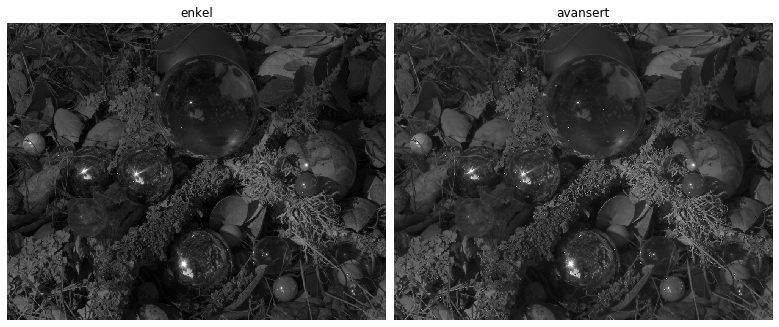
\includegraphics[width=1\columnwidth]{bilder/konvert.png}
    \caption{Konvertering til gråtone
    \label{fig:graytone}} 
\end{center}
\end{figure}



